\section{Задание 3}

Создайте документ, в котором одни рисунок занимает 50\% окна и является нижним слоем. На верхнем слое второй рисунок, который двигается по вертикали к нижней границе первого рисунка, затем на столбец (ширину рисунка) вправо и вверх, к верхней границе, на столбец вправо и к нижней границе, и т.д. до правой границы нижнего рисунка.

\begin{center}
  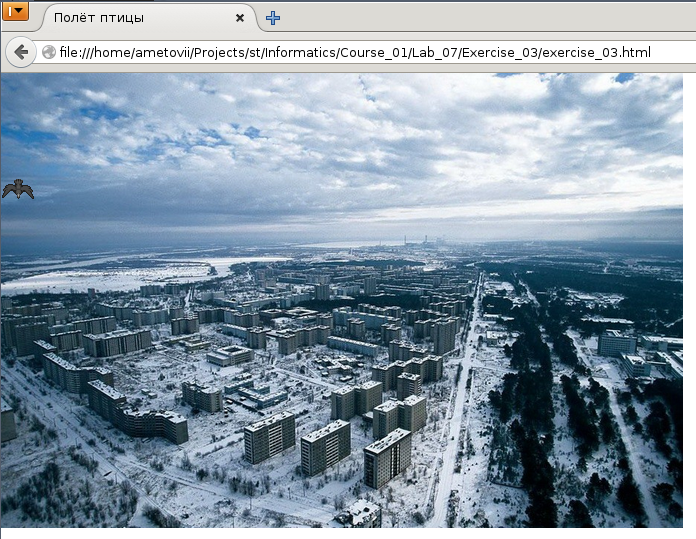
\includegraphics[width=10cm]{img/Exercise_03/01.png}
  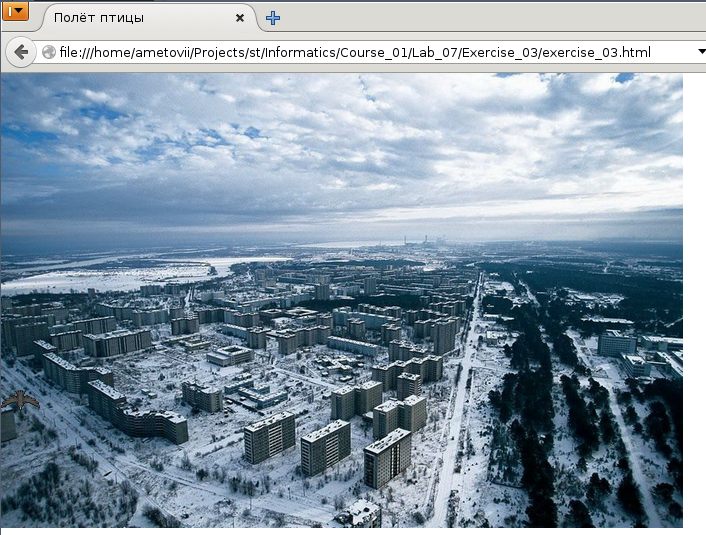
\includegraphics[width=10cm]{img/Exercise_03/02.png}
  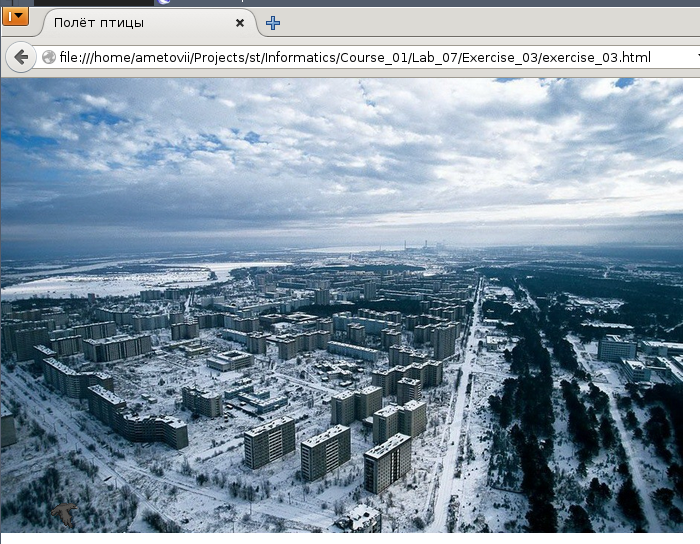
\includegraphics[width=10cm]{img/Exercise_03/03.png}
  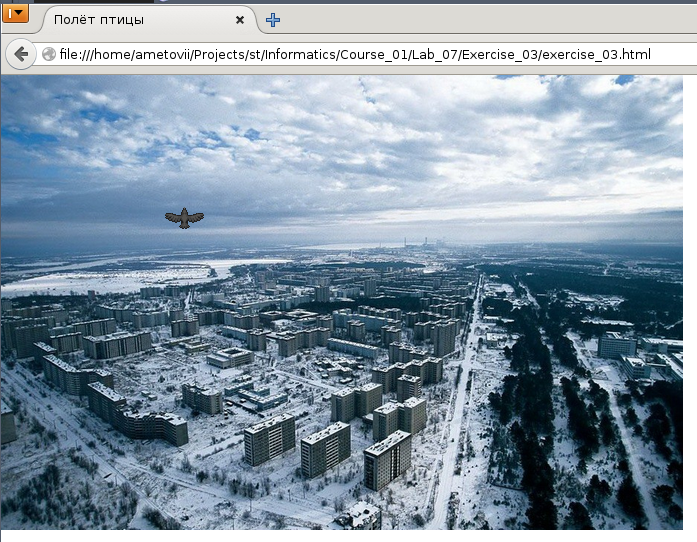
\includegraphics[width=10cm]{img/Exercise_03/04.png}
  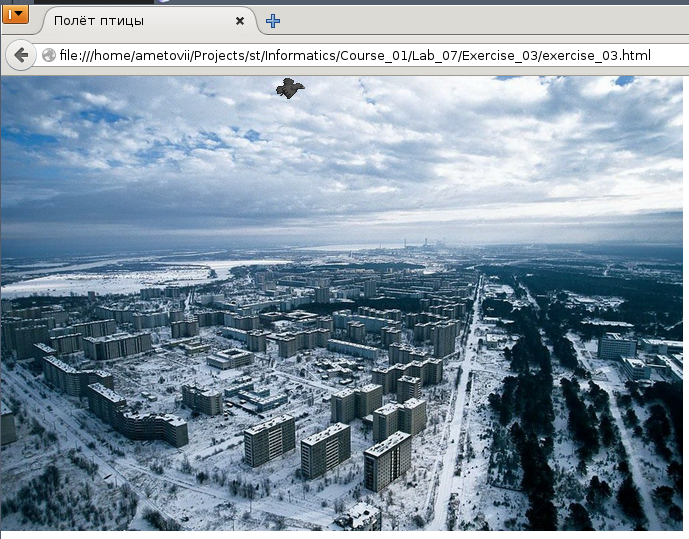
\includegraphics[width=10cm]{img/Exercise_03/05.png}
  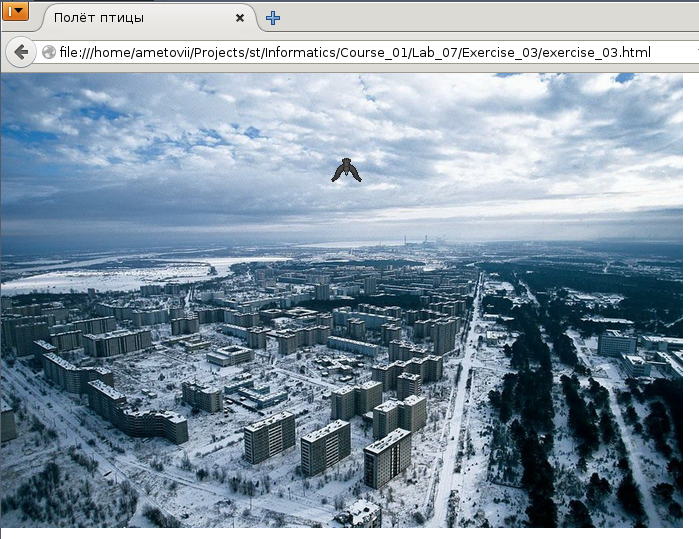
\includegraphics[width=10cm]{img/Exercise_03/06.png}
  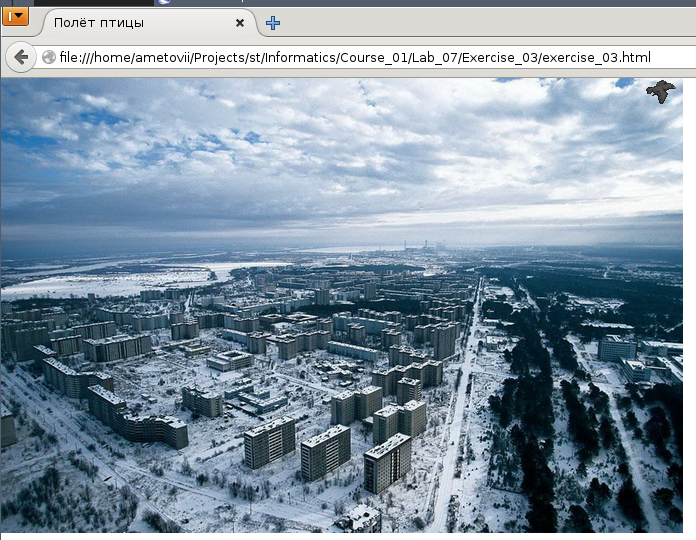
\includegraphics[width=10cm]{img/Exercise_03/07.png}
\end{center}

Исходный код \verb|exercise_03.html|:

\begin{verbatim}
<!DOCTYPE HTML>
<html>
  <head>
    <meta charset="utf-8">
    <title>Полёт птицы</title>
    <style type="text/css">
      .block1 {
      float: left;
      position: absolute;
      }
      
      .block2 {
          width: 50%;
          height: auto;
          float: left;
          position: absolute;
      }
    </style>
  </head>
  <body>
    <div class="block2" id='imageDiv' style="left:0px; top:0px;">
      <img src="Background/Pripyat.jpg" style="width:100%;"
	   id='Pripyat'>
    </div>
    <div class="block1" id='changedDiv'>
      <img id='bird' src="Sprites/ew_01.png" width="100%">
    </div>
        <script>
      currentSprite=0;
      currentTop=0;
      currentLeft=0;
      currentLocation=450;
      leftOffset=0;
      direction=1;
      // 1 - North-South
      // 2 - West-East
      // 3 - South-North
      // 4 - East-West
      
      function go(){
          currentSprite++;
          var myBird=document.getElementById('bird');
          var backgroundDiv=document.getElementById('imageDiv');
          switch (direction){
          case 1:
              currentTop=currentTop+4;
              myBird.src="Sprites/ns_0"+(currentSprite%5)+".png";
	      if (currentTop>=backgroundDiv.offsetHeight-35)
		  direction=2;
              break
          case 2:
              currentLeft=currentLeft+4;
              leftOffset++;
              myBird.src="Sprites/we_0"+(currentSprite%4)+".png";
	      if (leftOffset>40){
		  if (currentTop==0){
                      direction=1;
                      leftOffset=0;
                  }
                  else {
                      direction=3;
                      leftOffset=0;
                  }
              }
              break
          case 3:
              currentTop=currentTop-4;
              myBird.src="Sprites/sn_0"+(currentSprite%4)+".png";
              if (currentTop<=0) direction=2;
          default:
          }
          var myPripyat=document.getElementById('Pripyat');
          var birdDiv=document.getElementById('changedDiv');
	  birdDiv.style="left:"+currentLeft+"px; top:"+
	      currentTop+"px;";
	  if (currentLeft<backgroundDiv.offsetWidth-40)
	      setTimeout('go()', 80);
      }

      go();
    </script>
  </body>
</html>
\end{verbatim}
